%%%%%%%%%%%%%%%%%%%%%%%%%%%%%%%%%%%%%%%%%%%%%%
% An example of a lab report write-up.
%%%%%%%%%%%%%%%%%%%%%%%%%%%%%%%%%%%%%%%%%%%%%%
% This is a combination of several labs that I have done in the past for
% Computer Engineering, so it is not to be taken literally, but instead used as
% a great starting template for your own lab write up.  When creating this
% template, I tried to keep in mind all of the functions and functionality of
% LaTeX that I spent a lot of time researching and using in my lab reports and
% include them here so that it is fairly easy for students first learning LaTeX
% to jump on in and get immediate results.  However, I do assume that the
% person using this guide has already created at least a "Hello World" PDF
% document using LaTeX (which means it's installed and ready to go).
%
% My preference for developing in LaTeX is to use the LaTeX Plugin for gedit in
% Linux.  There are others for Mac and Windows as well (particularly MikTeX).
% Another excellent plugin is the Calc2LaTeX plugin for the OpenOffice suite.
% It makes it very easy to create a large table very quickly.
%
% Professors have different tastes for how they want the lab write-ups done, so
% check with the section layout for your class and create a template file for
% each class (my recommendation).
%
% Also, there is a list of common commands at the bottom of this document.  Use
% these as a quick reference.  If you'd like more, you can view the "LaTeX Cheat
% Sheet.pdf" included with this template material.
%
% (c) 2009 Derek R. Hildreth <derek@derekhildreth.com> http://www.derekhildreth.com
% This work is licensed under the Creative Commons Attribution-NonCommercial-ShareAlike License. To view a copy of this license, visit http://creativecommons.org/licenses/by-nc-sa/1.0/ or send a letter to Creative Commons, 559 Nathan Abbott Way, Stanford, California 94305, USA.
%%%%%%%%%%%%%%%%%%%%%%%%%%%%%%%%%%%%%%%%%%%%%%
\documentclass[aps,letterpaper,10pt]{revtex4}
\input kvmacros % For Karnaugh Maps (K-Maps)

\usepackage{graphicx} % For images
\usepackage{float}    % For tables and other floats
\usepackage{verbatim} % For comments and other
\usepackage{amsmath}  % For math
\usepackage{amssymb}  % For more math
\usepackage{fullpage} % Set margins and place page numbers at bottom center
\usepackage{listings} % For source code
\usepackage{subfig}   % For subfigures
\usepackage[usenames,dvipsnames]{color} % For colors and names
\usepackage[pdftex]{hyperref}           % For hyperlinks and indexing the PDF
\hypersetup{ % play with the different link colors here
    colorlinks,
    citecolor=blue,
    filecolor=blue,
    linkcolor=blue,
    urlcolor=blue % set to black to prevent printing blue links
}

\definecolor{mygrey}{gray}{.96} % Light Grey
\lstset{
	language=[ISO]C++,              % choose the language of the code ("language=Verilog" is popular as well)
   tabsize=3,							  % sets the size of the tabs in spaces (1 Tab is replaced with 3 spaces)
	basicstyle=\tiny,               % the size of the fonts that are used for the code
	numbers=left,                   % where to put the line-numbers
	numberstyle=\tiny,              % the size of the fonts that are used for the line-numbers
	stepnumber=2,                   % the step between two line-numbers. If it's 1 each line will be numbered
	numbersep=5pt,                  % how far the line-numbers are from the code
	backgroundcolor=\color{mygrey}, % choose the background color. You must add \usepackage{color}
	%showspaces=false,              % show spaces adding particular underscores
	%showstringspaces=false,        % underline spaces within strings
	%showtabs=false,                % show tabs within strings adding particular underscores
	frame=single,	                 % adds a frame around the code
	tabsize=3,	                    % sets default tabsize to 2 spaces
	captionpos=b,                   % sets the caption-position to bottom
	breaklines=true,                % sets automatic line breaking
	breakatwhitespace=false,        % sets if automatic breaks should only happen at whitespace
	%escapeinside={\%*}{*)},        % if you want to add a comment within your code
	commentstyle=\color{BrickRed}   % sets the comment style
}

% Make units a little nicer looking and faster to type
\newcommand{\Hz}{\textsl{Hz}}
\newcommand{\KHz}{\textsl{KHz}}
\newcommand{\MHz}{\textsl{MHz}}
\newcommand{\GHz}{\textsl{GHz}}
\newcommand{\ns}{\textsl{ns}}
\newcommand{\ms}{\textsl{ms}}
\newcommand{\s}{\textsl{s}}



% TITLE PAGE CONTENT %%%%%%%%%%%%%%%%%%%%%%%%
% Remember to fill this section out for each
% lab write-up.
%%%%%%%%%%%%%%%%%%%%%%%%%%%%%%%%%%%%%%%%%%%%%
\newcommand{\labno}{05}
\newcommand{\labtitle}{AU 332 Artificial Intelligence: Principles and Techniques}
\newcommand{\authorname}{WangChunhui (517021910047)}
\newcommand{\hw}{1}
% END TITLE PAGE CONTENT %%%%%%%%%%%%%%%%%%%%


\begin{document}  % START THE DOCUMENT!


% TITLE PAGE %%%%%%%%%%%%%%%%%%%%%%%%%%%%%%%%%%%%%%
% If you'd like to change the content of this,
% do it in the "TITLE PAGE CONTENT" directly above
% this message
%%%%%%%%%%%%%%%%%%%%%%%%%%%%%%%%%%%%%%%%%%%%%%%%%%%
\begin{titlepage}
\begin{center}
{\Large \textsc{\labtitle} \\ \vspace{4pt}}
\rule[13pt]{\textwidth}{1pt} \\ \vspace{150pt}
{\large By: \authorname \\ \vspace{10pt}
HW\#: \hw \\ \vspace{10pt}
\today}
\end{center}
\end{titlepage}
% END TITLE PAGE %%%%%%%%%%%%%%%%%%%%%%%%%%%%%%%%%%





%%%%%%%%%%%%%%%%%%%%%%%%%%%%%%
%%%%%%%%%%%%%%%%%%%%%%%%%%%%%%
\section{Introduction}
%No Text Here
%%%%%%%%%%%%%%%%%%%%%%%%%%%%%%%
\subsection{Purpose}
\begin{comment}
This is a lab template which has a ton of different things which are useful in writing lab write-ups in the Computer Eningeering field.  This is demonstrating the comment block. Don't be overwhelmed, it may seem like a lot to take in at a time, but it's worth spending the time learning it.
\end{comment}
The goal of today’s lab is to re-design the LED/Switch system (delivered to students in the LEDTest1 programs) to include a hardware timer.  This lab will entail updating the software to be able to configure the timer unit and respond to timer interrupts.  Instead of using a delay loop for the timing of the LED’s, students need to configure a timer unit on the BF533 to provide accurate timing.  When the timer times out, the timer should generate an interrupt and the software should respond to that interrupt by blinking the LED’s. \vspace{3mm} % I use this to seperate the paragraphs a bit.

In this lab, students will use a round-robin with interrupt software architecture using the \texttt{LEDTest1.c} example program as the basis for the design.  The software needs to do 4 main functions.  First the SW needs to be able to initialize the peripheral units (timer and programmable flags).  Second the SW needs to be able to respond to button.  Third the SW needs to be able to respond to timer interrupts.  And fourth, the SW needs to be able to control the LED’s per the buttons and the timer interrupt.
From an architectural standpoint, the SW can be broken into 4 main sections:
\begin{itemize}
	\item LED Control -- functions to control the LED's
	\item Interrupt -- ISR
	\item Timer Control -- functions to control the timer units
	\item Main Loop
\end{itemize}
\vspace{3mm}

Students will need one timer interrupt.  In this interrupt, they should set a flag indicating that the ISR was asserted.
The main control SW needs to be able to do 2 things.  First it needs to initialize the timer unit, the programmable flags and the interrupt.  Next it needs to read the button press, the flags updated by the ISR’s, and output the correct LED’s.

%%%%%%%%%%%%%%%%%%%%%%%%%%%%%%
\subsection{Equipment}
There is a minimal amount of equipment to be used in this lab.  The few requirements are listed below:
	\begin{itemize}
		\item Xilinx ISE Navigator Software (v10.0.1)
		\item Computer capable of running the software mentioned
		\item Spartan 3E FPGA Developer Board (For Hardware Simulation)
	\end{itemize}

%%%%%%%%%%%%%%%%%%%%%%%%%%%%%%
\subsection{Procedure}

	\begin{enumerate}
		\item Start the ISE Navigator. See the ISE 8.2i Quick Start Tutorial.
		\item Create a new project.
		\item Import copies of the Verilog modules AND\_OR, MY\_AND2, and MY\_OR2 to the new project just created.
		\item Create a Test Bench (called Test Fixture in Verilog).
		\item Create the actual input stimulus.
		\item Run the simulation, examine the waveforms, and verify functioniality.
	\end{enumerate}

%%%%%%%%%%%%%%%%%%%%%%%%%%%%%%
%%%%%%%%%%%%%%%%%%%%%%%%%%%%%%
\newpage
\section{Schematic Diagrams}
This section consists of screenshots taken during the laboratory procedure.  One set of the screenshots is of the periods captured by the oscilliscope and the other set is captured by the logic analyzer.

	% You can refer to this set of images by using \ref{fig:oscil}.  ie "please refer to Figure \ref{fig:oscil}."
	% You can refer to a specific subimage by using \ref{fig:Per6A}. ie "please refer to Figure \ref{fig:Per6A}."
   % I prefer the quality of a .png image, but you may use other extensions such as .jpg.
	\begin{figure}[H]
	  \centering
	  \subfloat[LED4 Period]{\label{fig:Per6A}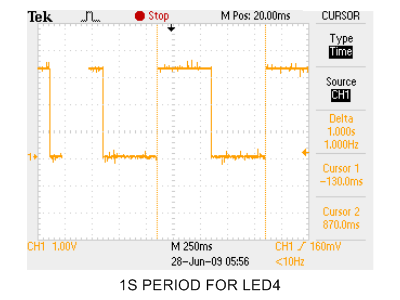
\includegraphics[width=0.4\textwidth]{period_led4.png}} \\
	  \subfloat[LED5 Period]{\label{fig:Per6A}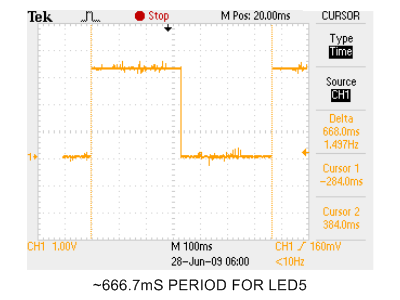
\includegraphics[width=0.4\textwidth]{period_led5.png}}
	  \subfloat[LED6 Period]{\label{fig:Per6A}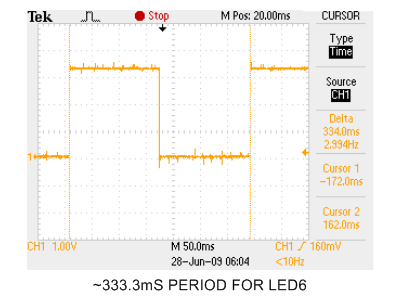
\includegraphics[width=0.4\textwidth]{period_led6.png}}
	  \caption{Period of LED blink rate captured by osciliscope.}
	  \label{fig:oscil}
	\end{figure}

%%%%%%%%%%%%%%%%%%%%%%%%%%%%%%
%%%%%%%%%%%%%%%%%%%%%%%%%%%%%%
\newpage
\section{Experiment Data}
This section will consist of the important code blocks which were changed in order to meet the requirements of the lab.  \vspace{5mm}
	\lstinputlisting{code.c}
	\vspace{3mm}

% IF YOU'D RATHER TYPE THE CODE, OR HAVE A SMALLER BLOCK OF CODE, USE THIS:
%\begin{lstlisting}
%if(something)
%	do this
%else
%	do this
%\end{lstlisting}

%% THIS IS FROM A DIFFERENT CLASS, BUT DEMONSTRATES MATH MODE WELL
%%%%%%%%%%%%%%%%%%%%%%%%%%%%%%
\subsection{Formulas and Overall Descriptions Used}
This part of the laboratory was done for \href{http://www.byui.edu/catalog/2004-2005/class.asp1075.htm}{Feedback Control}.  Most of this laboratory's calculations were completed and compiled by the folks at Quanser (the manufacturer of the inverted pendulum) and will give the lab a good starting place.  Below are the state equation and gain values used initially in the lab:
	\[
	\begin{bmatrix}
	\dot{\alpha} \\
	\ddot{\alpha} \\
	\dot{\theta} \\
	\ddot{\theta} \\
	\end{bmatrix}
	=
	\begin{bmatrix}
	0 & 1 & 0 & 0 \\
	81.7 & 0 & 0 & -13.9 \\
	0 & 0 & 0 & 1 \\
	39.7 & 0 & 0 & -14.4 \\
	\end{bmatrix}
	\begin{bmatrix}
	\alpha \\
	\dot{\alpha} \\
	\theta \\
	\dot{\theta} \\
	\end{bmatrix}
	+
	\begin{bmatrix}
	0 \\
	24.5 \\
	0 \\
	25.4 \\
	\end{bmatrix}
	V
	\]

	\[
	K  =
	\begin{bmatrix}
	21 & 2.8 & -2.2 & -2.0 \\
	\end{bmatrix}
	\]

Other values, such as the $\frac{\mbox{Volts}}{\mbox{Degree}}$ and $\frac{\mbox{Degrees}}{\mbox{Volt}}$ were obtained by first determining the max angle of the pendulum on both extreme sides.

Using the max angles from above, these values were determined:
	\[
	\begin{array}{l l}
		\alpha = 0.062 \frac{\mbox{Volts}}{\mbox{Degree}} \\ \\
		\alpha = 15.105 \frac{\mbox{Degrees}}{\mbox{Volt}} \\
	\end{array}
	\]

I would also like to add that in order to calibrate $\alpha$ to get a perfect vertical $= 0$, a value of $0.09$ needed to be added.  The same applies to $\theta$ where $0.322$ needs to be added.

%%%%%%%%%%%%%%%%%%%%%%%%%%%%%%
\subsection{DC Motor Transfer Function and Parameters}

Definitions:
	\begin{align*}
		\theta(t) =  Angular Position \\
		\dot{\theta}(t) =  Angular Velocity \\
		\triangle t = t_{10\%} - t_{90\%} \\
		90\% = e^{-t_{10\%}/\tau} \\
		10\% = e^{-t_{90\%}/\tau} \\
	\end{align*}

The Math:
	\begin{align*}
		\frac{s\theta(s)}{V_{a}(s)} = \frac{K}{s+P} \\
		\mbox{Let}\ V_{a}(s) = \frac{V_{0}}{s} \\  % If you'd like to have a space following any command, add "\" to the end as shown here.
		s\theta(s) = \frac{KV_{0}}{(S+P)S} = \frac{KV_{0}}{\frac{P}{S}} - \frac{\frac{KV_{0}}{P}}{s+P} \\
		L^{-1} \Rightarrow \dot{\theta}(t) = \frac{KV_{0}}{P}(1-e^{-t/(1/P)}) \\
		\dot{\theta}(t) = (\dot{\theta}_{i} - \dot{\theta}_{f})e^{-pt} + \dot{\theta}_{f} \\
	\end{align*}

Final equations:
	\begin{align}
		\label{thetadot}\dot{\theta}_{f} = \frac{KV_{0}}{P} \\
		\label{equ:tau}\frac{1}{P} = \tau = \frac{\triangle t}{ln(9)}
	\end{align}

Graphically (Refer to Equation \ref{thetadot} and Equation \ref{equ:tau}) :
	% Drawn and exported to png using Inkscape.
	\begin{figure}[h]
		\begin{center}
			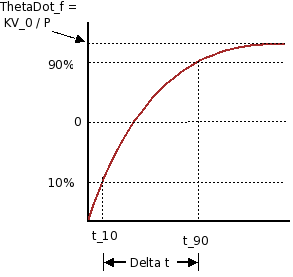
\includegraphics[width=0.33\textwidth]{graph.png}
		\end{center}
	\label{graph}
	\end{figure}

% AGAIN, ANOTHER EXAMPLE FROM A DIFFERENT CLASS WHICH DEMONSTRasdATES KMAPS AND TABLES NICELY.
\newpage % I added this after viewing the completed pdf and decided to make this cosmetic change
This section consists of tables and reductions which were used in this laboratory exercise.

% This table was generated using the Calc2LaTeX macro which I mentioned earlier.
% You'll need OpenOffice installed and you'll have to download the macro online.
% If you're interested, I have a guide on how to set this up and use it on my
% blog.  http://www.derekhildreth.com/blog  Search for "LaTeX".  You'll find it.
	\begin{table}[htbp]
	\begin{center}
		\begin{tabular}{|ccc|cc|}
			\hline
			\textbf{PS} & \textbf{D} & \textbf{N} & \textbf{NS} & \textbf{P} \\ \hline
			\$0.00 & 0 & 0 & \$0.00 & 0 \\
			 & 0 & 1 & \$0.05 & 0 \\
			 & 1 & 0 & \$0.10 & 0 \\
			 & 1 & 1 & -- & -- \\ \hline
			\$0.05 & 0 & 0 & \$0.05 & 0 \\
			 & 0 & 1 & \$0.10 & 0 \\
			 & 1 & 0 & \$0.15 & 0 \\
			 & 1 & 1 & -- & -- \\ \hline
			\$0.10 & 0 & 0 & \$0.10 & 0 \\
			 & 0 & 1 & \$0.15 & 0 \\
			 & 1 & 0 & \$0.15 & 0 \\
			 & 1 & 1 & -- & -- \\ \hline
			\$0.15 & -- & -- & \$0.15 & 1 \\ \hline
			\end{tabular}
	\end{center}
	\caption{Symbolic Transition Table}
	\label{symbolic}
	\end{table}

	\begin{table}[H]
		\centering
		\subfloat[D1 = $Q_{1}$+D+$Q_{0}$N] % Caption
			{
				\karnaughmap{4}{D1:}{ {$Q_{1}$} {$Q_{0}$} {D} {N} }{001X011X111X111X}{}  % See the included kvdoc.pdf file for more details
			} \hspace{10mm} % seperate them a bit
		\subfloat[D0 = $\Bar{Q_{0}}$N + $Q_{0}\Bar{N}$ + $Q_{1}$N + $Q_{1}$D] % Caption
			{
				\karnaughmap{4}{D0:}{ {$Q_{1}$} {$Q_{0}$} {D} {N} }{010X101X011X111X}{}
			}
	  \caption{Karnaugh maps and the simplified results of the logic.}
	  \label{fig:kmaps}
	\end{table}


%%%%%%%%%%%%%%%%%%%%%%%%%%%%%%
%%%%%%%%%%%%%%%%%%%%%%%%%%%%%%
\newpage
\section{Discussion \& Conclusion}
The goal of this lab was to re-design the LED/Switch system to include a hardware timer.  By pressing eight different combinations of the three buttons, the LEDs on the board were to act in different ways using these timers. There was not a Q\&A requirement for this lab. \vspace{3mm} % I use this to seperate the paragraphs a bit.

I was able to accomplish the requirements of the lab by utilizing the \texttt{IntMgrTimerExample.c} project found within the analog devices example programs folder (and mentioned in the class lecture).  There were some stumbling blocks to overcome.  The most difficult for myself was actually getting the period of the LEDs just right.  I was able to get it very close to the 333.3\ms, 666.7\ms, and 1\s periods, but not exactly.  My first method of getting these periods right was to take the clock speed in \MHz, find the period by taking the inverse of the clock speed, and then solving for the value in hex that was needed to get the right period.  This didn't yeild very accurate results at all, and so I then went through a trial and error session until I got a value of 1.1\ms.  I used this value in hex to calculate the other periods.  The results of this method can be seen in Figure \ref{fig:oscil} above in the schematics section. \vspace{3mm}

Another observation I would like to point out is that I put all of my logic within the interrupts themselves.  I feel that this was a hacked way of doing the lab to save time and that it's probably not the best programming method.  After I was completed with my lab, I viewed other students solutions and they just seemed more elegant.  Interestingly enough, the other students weren't incredibly happy with their solution either.  If I were to go back and do this lab again, I would invest more time in both understanding how to utilze the interrupts as well as find a more elegant solution to blink the lights. \vspace{3mm}

All in all, this laboratory gave me an insight on how interrupts work and I hope to be able to apply them to following labs\ldots


\end{document} % DONE WITH DOCUMENT!


%%%%%%%%%%
PERSONAL FAVORITE LAB WRITE-UP STRUCTURE
%%%%%%%%%%
\section{Introduction}
	% No Text Here
	\subsection{Purpose}
		% Lab objective
	\subsection{Equipment}
		% Any and all equipment used (specific!)
	\subsection{Procedure}
		% Overview of the procedure taken (not-so-specific!)
\newpage
\section{Schematic Diagrams}
	% Any schematics, screenshots, block
   % diagrams used.  Possibly photos or
	% images could go here as well.
\newpage
\section{Experiment Data}
	% Depending on lab, program code would be
	% included here without the Estimated and
	% Actual Results.
	\subsection{Estimated Results}
		% Calculated. What it should be.
	\subsection{Actual Results}
		% Measured.  What it actually was.
\newpage
\section{Discussion \& Conclusion}
	% 3 Paragraphs:
		% Restate the objective of the lab
		% Discuss personal trials, errors, and difficulties
		% Conclude the lab


%%%%%%%%%%%%%%%%
COMMON COMMANDS:
%%%%%%%%%%%%%%%%
% IMAGES
begin{figure}[H]
   \begin{center}
      \includegraphics[width=0.6\textwidth]{RTL_SCHEM.png}
   \end{center}
\caption{A screenshot of the RTL Schematics produced from the Verilog code.}
\label{RTL}
\end{figure}

% SUBFIGURES IMAGES
\begin{figure}[H]
  \centering
  \subfloat[LED4 Period]{\label{fig:Per4}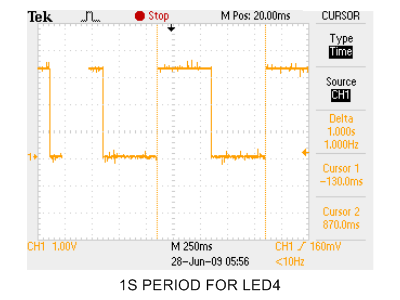
\includegraphics[width=0.4\textwidth]{period_led4.png}} \\
  \subfloat[LED5 Period]{\label{fig:Per5}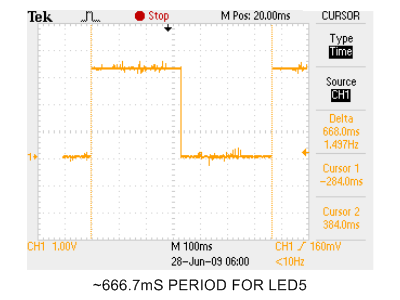
\includegraphics[width=0.4\textwidth]{period_led5.png}}
  \subfloat[LED6 Period]{\label{fig:Per6}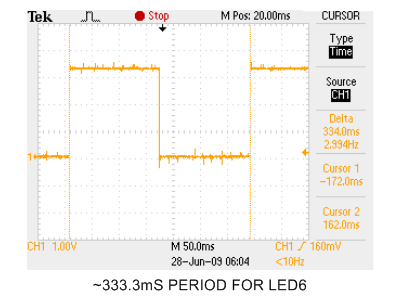
\includegraphics[width=0.4\textwidth]{period_led6.png}}
  \caption{Period of LED blink rate captured by osciliscope.}
  \label{fig:oscil}
\end{figure}

% INSERT SOURCE CODE
\lstset{language=Verilog, tabsize=3, backgroundcolor=\color{mygrey}, basicstyle=\small, commentstyle=\color{BrickRed}}
\lstinputlisting{MODULE.v}

% TEXT TABLE
\begin{table}
\begin{center}
\begin{tabular}{|l|c|c|l|}
	x & x & x & x \\ \hline
	x & x & x & x \\
	x & x & x & x \\ \hline
\end{tabular}
\caption{Caption}
\label{label}
\end{center}
\end{table}

% MATHMATICAL ENVIRONMENT
$ 8 = 2 \times 4 $

% CENTERED FORMULA
\[  \]

% NUMBERED EQUATION
\begin{equation}
	
\end{equation}

% ARRAY OF EQUATIONS (The splat supresses the numbering)
\begin{align*}
	
\end{align*}

% NUMBERED ARRAY OF EQUATIONS
\begin{align}
	
\end{align}

% ACCENTS
\dot{x} % dot
\ddot{x} % double dot
\bar{x} % bar
\tilde{x} % tilde
\vec{x} % vector
\hat{x} % hat
\acute{x} % acute
\grave{x} % grave
\breve{x} % breve
\check{x} % dot (cowboy hat)

% FONTS
\mathrm{text} % roman
\mathsf{text} % sans serif
\mathtt{text} % Typewriter
\mathbb{text} % Blackboard bold
\mathcal{text} % Caligraphy
\mathfrak{text} % Fraktur

\textbf{text} % bold
\textit{text} % italic
\textsl{text} % slanted
\textsc{text} % small caps
\texttt{text} % typewriter
\underline{text} % underline
\emph{text} % emphasized

\begin{tiny}text\end{tiny} % Tiny
\begin{scriptsize}text\end{scriptsize} % Script Size
\begin{footnotesize}text\end{footnotesize} % Footnote Size
\begin{small}text\end{small} % Small
\begin{normalsize}text\end{normalsize} % Normal Size
\begin{large}text\end{large} % Large
\begin{Large}text\end{Large} % Larger
\begin{LARGE}text\end{LARGE} % Very Large
\begin{huge}text\end{huge}   % Huge
\begin{Huge}text\end{Huge}   % Very Huge


% GENERATE TABLE OF CONTENTS AND/OR TABLE OF FIGURES
% These seem to have some issues with the "revtex4" document class.  To use, change
% the very first line of this document to "article" like this:
% \documentclass[aps,letterpaper,10pt]{article}
\tableofcontents
\listoffigures
\listoftables

% INCLUDE A HYPERLINK OR URL
\url{http://www.derekhildreth.com}
\href{http://www.derekhildreth.com}{Derek Hildreth's Website}

% FOR MORE, REFER TO THE "LINUX CHEAT SHEET.PDF" FILE INCLUDED!
